\documentclass{article}

\usepackage[margin=2.5cm]{geometry}

\usepackage[utf8]{inputenc}
\usepackage{amsfonts} 
\usepackage{array} 
\usepackage{enumitem}
\usepackage{tabularx}
\usepackage{graphicx}
\usepackage{fancyhdr}
\usepackage{fancyvrb}
\usepackage{amsmath}
\usepackage{amsthm}
\usepackage[most]{tcolorbox}
\tcbuselibrary{breakable}
\usepackage{float}
\usepackage{listings}  
\usepackage{xcolor}
\usepackage{subfigure}
\usepackage[htt]{hyphenat}

\definecolor{codegreen}{rgb}{.2,0.6,0}
\definecolor{codegray}{rgb}{0.5,0.5,0.5}
\definecolor{codepurple}{rgb}{0.58,0,0.82}
\definecolor{codeblue}{rgb}{0,0.4,0.82}
\definecolor{codeorange}{rgb}{0.94,0.34,0.0}
\definecolor{backcolour}{rgb}{0.95,0.95,0.92}
\definecolor{backcolourgray}{rgb}{0.92,0.92,0.92}
\definecolor{codewhite}{rgb}{1,1,1}

\lstdefinestyle{mystyle}{
    backgroundcolor=\color{backcolourgray},   
    commentstyle=\color{codegreen},
    keywordstyle=\color{codeblue},
    numberstyle=\tiny\color{black},
    stringstyle=\color{codeorange},
    basicstyle=\ttfamily\footnotesize,
    breakatwhitespace=false,         
    breaklines=true,                 
    captionpos=b,                    
    keepspaces=true,                 
    %numbers=left,                    
    numbersep=5pt,                  
    showspaces=false,                
    showstringspaces=false,
    showtabs=false,                  
    tabsize=2,
    extendedchars=true,
    frame=single
    %, basicstyle=\footnotesize
}
\lstset{style=mystyle}

\usepackage{hyperref}
\hypersetup{
    colorlinks=true,
    linkcolor=blue,
    filecolor=magenta,      
    urlcolor=cyan,
}

\pagestyle{fancy}
\fancyhf{}
\rhead{AI. Practice 1.}
\lhead{Pablo Cuesta Sierra, Álvaro Zamanillo Sáez - G2351, P05}
\cfoot{\thepage}

\usepackage{titlesec}
%\titleformat*{\subsection}{\large\bfseries\color{darkgray}}
%\titleformat*{\subsubsection}{\normalsize\itshape\color{darkgray}}

%\setlength{\parskip}{0.15cm}


%parameters: file, caption, label, scale
\newcommand{\myFigure}[4]{%
    \begin{figure}[H]
        \includegraphics[width=#4\textwidth]{#1}
        \centering
        \caption{#2}
        \label{#3}
    \end{figure}
}

%grey item for enumerate
%\renewcommand{\thesubsubsection}{(\thesubsection.\alph{subsubsection})}
\setcounter{secnumdepth}{4}
\setcounter{tocdepth}{2}
%\newcommand{\question}[1]{\subsection{#1}}
%\newcommand{\subquestion}[1]{\subsubsection{#1}}


\setcounter{section}{0}


\begin{document}


\title{\textbf{Artificial Intelligence. Practice 1.}}
\author{\textbf{Pablo Cuesta Sierra, Álvaro Zamanillo Sáez} \\Group 2351. Pair 5.}
%\date{}
\maketitle

\begin{tcolorbox}
\tableofcontents
\end{tcolorbox}


\newpage
\section{Question 1: Finding a Fixed Food Dot using Depth First Search}

\subsection{Personal comment on the approach and decisions of the proposed solution (0.5pt)}\label{search_function}

In order to make the following questions easier, we have decided to abstract the notion of node and make a single generic search function where the type of container used to implement the \emph{openList} determines which algorithm is performed. 

%[language=C, texcl=true]
\begin{lstlisting} [captionpos=t,caption={Generic algorithm (taken from the AI theory slides)}]
    function Tree-Search (problem, strategy )
        ;; returns solution or fail
        ;; opened-list contains the nodes in the fringe of the search tree
        Initialize search-tree with root-node
        Initialize opened-list with root-node
        Iterate
            If (opened-list is empty) then return fail
            Choose from opened-list, according to strategy, a node to expand.
                If (node satisfies goal-test )
                    then return solution (path from root-node to current node )
                else remove node from opened-list
                    expand node
                    add child nodes to opened-list 
\end{lstlisting}


\subsubsection{List \& explanation of the framework functions used}

\begin{itemize}
    \item The \texttt{Node} class, with methods:
    \begin{itemize}
        \item \texttt{\_\_init\_\_(self, state, action, cost, parentNode)}
        \item \texttt{path(self)}
        \item \texttt{\_\_eq\_\_(self, \_\_o)}
    \end{itemize}
    \item \texttt{expandNode(problem , node , openList , closedList)}
    \item \texttt{search(problem, openList)}
    \item \texttt{depthFirstSearch(problem)}
\end{itemize}

For the generic function (\texttt{search}), we have used the implementation of `containers' done in the \emph{util.py} file (\emph{Stack}, \emph{Queue}, \emph{PriorityQueueWithFunction}), which have the methods \emph{pop()} and \emph{push()}. Also, to initialize the elements of the search, we have to use the \emph{SearchProblem} class methods, to get the start state, the successors of a state and whether a state is a goal state.

For the algorithm, we had to choose a structure for the nodes of the graph search. Each node contains a game state, the last action taken to get to that state, the cost of the path that goes from the start to this state, and a pointer to its parent node. In order to compare nodes, as we are implementing graph search and do not want to expand two nodes that have the same state, we consider that two nodes are equal if their states are equal.

The node also has a method that calculates the path taken from the root to that node, which goes up the tree using the reference to the parent to build this list of actions. Another implementation would have been to keep only state and path, for each node. However, each time we concatenate a new action to the path list of a node to create a successor, the list would have to be copied (\texttt{new\_list = prev\_list + [new\_action]}), which means a high cost both in terms of time and space efficiency: there is a cost of $\mathcal{O}(N)$ for each operation of that kind. Our implementation has a $\mathcal{O}(N)$ cost ($N$ being the size of the final list), but the path is only computed once in the whole search algorithm (when the solution is found). 

This particular algorithm, \emph{DFS}, requires the `openList' to be a stack.

\subsubsection{Includes code written by students}

\begin{lstlisting}[language=python, caption = The Node class (\emph{search.py}),captionpos=t]
    class Node:
        '''
            Node class: nodes used for the tree of the search function.
                state: state of the problem
                action: last action taken from the predecessor of the state to get to this state
                cost: total cost from the root to this state
                parentNode: points to the parent node
                path: list of actions from the root to the node 
        '''

        def __init__(self, state, action, cost, parentNode):
            self.state = state
            self.action = action
            self.cost = cost
            self.parentNode = parentNode

        @property
        def path(self):
            '''
                The path from the node to the root.
                Returns the list of actions from the beginning to the node.
            '''
            node,actions=self,[]

            while node.parentNode != None:
                actions.insert(0,node.action)
                node = node.parentNode
            return actions
        
        def __eq__(self, __o):
            if isinstance(__o, Node):
                return __o.state == self.state
            return False
\end{lstlisting}

\begin{lstlisting}[language=python, captionpos=t, caption = {The search function (\emph{search.py})}]
    def expandNode(problem, node, openList, closedList):
        '''
            Expands a node for the search algorithm
                problem: problem to be solved by the search function
                node: node to be expanded
                openList: openList of the algorithm
                closedList: container of the search function
        '''
        closedList.append(node)
        for successor in problem.getSuccessors(node.state):
            openList.push(Node(
                            state=successor[0],
                            action=successor[1],
                            cost=successor[2]+node.cost, 
                            parentNode=node))

    def search(problem, openList):
        '''
            Search function that generalizes the different search types. 
                problem: problem to solve
                openList: the empty openList to be used in the implementation.
        '''
        closedList = []
        openList.push(Node(
                state=problem.getStartState(), 
                action=None, 
                cost=0, 
                parentNode=None))  # root node

        while not openList.isEmpty(): 
            currentNode = openList.pop()
            if problem.isGoalState(currentNode.state):
                return currentNode.path
            if currentNode not in closedList:
                expandNode(problem, currentNode, openList, closedList)
        
        return [] # No solution found  
\end{lstlisting}


\begin{lstlisting}[language=python, captionpos=t, caption={The \emph{DFS} function (\emph{search.py})}]
    def depthFirstSearch(problem):
        """Search the deepest nodes in the search tree first."""
        return search(problem, util.Stack())
\end{lstlisting}

\subsubsection{Screenshots of executions and test carried out analyzing the results}

\myFigure{./img/ex1/victoryDFS}{Results of the three tests using DFS}{victoryDFS}{.8}

\begin{figure}[H]
    \centering
    \subfigure[]{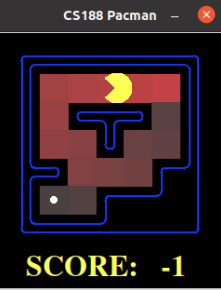
\includegraphics[height=0.291\textwidth]{./img/ex1/DFStiny}} 
    \subfigure[]{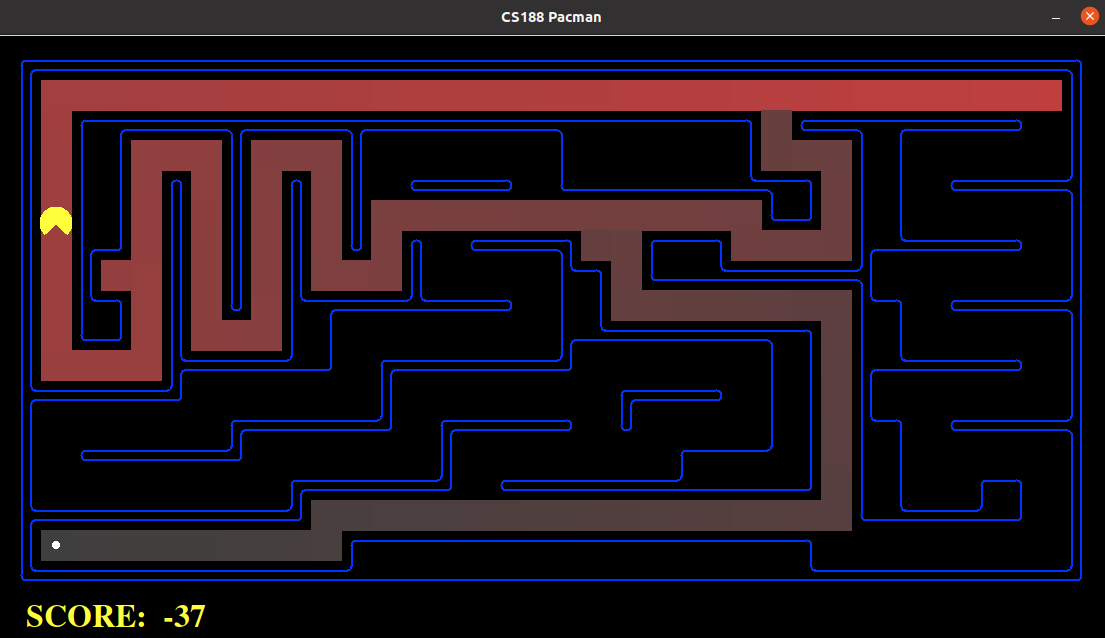
\includegraphics[height=0.291\textwidth]{./img/ex1/DFSmedium.png}} 
    \subfigure[]{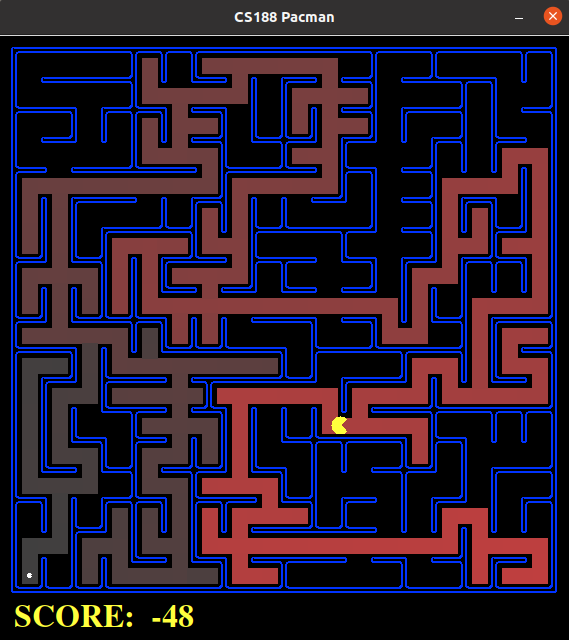
\includegraphics[height=0.291\textwidth]{./img/ex1/DFSbig.png}}
    \caption{Exploration for mazes with \emph{DFS}: \emph{tinyMaze}, \emph{mediumMaze} and \emph{bigMaze}.}
    \centering
    \label{exploration_e1}
\end{figure}

\myFigure{./img/ex1/test1}{Results of the autograder tests}{test1}{.7}

\subsection{Conclusions on the behavior of Pacman, it is optimal (y/n), reaches the solution (y/n), nodes that it expands, etc (0.5pt)}
\subsubsection{Answer to question 1.1: Is the exploration order what you would have expected? Does Pacman actually go to all the explored squares on his way to the goal?}
First of all, we notice (by looking at the code of the function \texttt{getSuccessors} in \textit{searchAgents.py}) that the order in which the children are generated is \texttt{(NORTH,SOUTH,EAST,WEST)}. Therefore, when using \textit{DFS} we expect that the algorithm explores all the way north until it reaches a wall, then all the way east (if it goes south, it will be a duplicate state) and so on. 

On the other hand, tiles explored by the algorithm but belonging to a branch that does not resolute, are not visited by Pacman.

This two behaviours are clearly shown in the screenshots of the tests (figure \ref{exploration_e1}).

\subsubsection{Answer to question 1.2: Is this a least cost solution? If not, think about what depth-first search is doing wrong.}

DFS is not optimal. The problem lies on the fact that the solution provided by DFS is the first branch visited which reachs the goal node; however, it is likely to happen that there exists another branch which is sorter and also leads to the solution.

\pagebreak

\section{Question 2: Breadth First Search}


\subsection{Personal comment on the approach and decisions of the proposed solution (0.5pt)}

Having done in the previous question the generic search algorithm, we just have to use the same algorithm, in this case with the `openList' being a queue (LIFO).

\subsubsection{List \& explanation of the framework functions used}

\begin{itemize}
    \item \texttt{breadthFirstSearch(problem)}
\end{itemize}

We used the \texttt{search()} function explained in the previous section (\ref{search_function}), along with the \emph{util.Queue} class for the open list.

\subsubsection{Includes code written by students}

\begin{lstlisting}[language=python,captionpos=t,caption={The \emph{BFS} function (\emph{search.py})}]
    def breadthFirstSearch(problem):
        """Search the shallowest nodes in the search tree first."""
        return search(problem, util.Queue())
\end{lstlisting}

\subsubsection{Screenshots of executions and test carried out analyzing the results}

\myFigure{./img/ex2/victoryBFS}{Results of the three tests using BFS}{victoryBFS}{.8}

\begin{figure}[H]
    \centering
    \subfigure[]{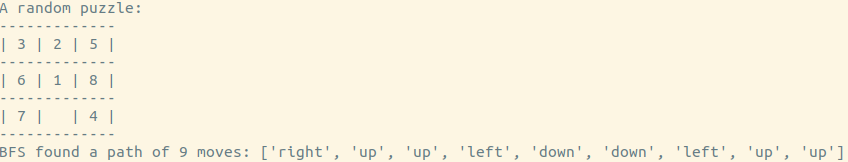
\includegraphics[width=.8\textwidth]{./img/ex2/8p_0}} 
    \subfigure[]{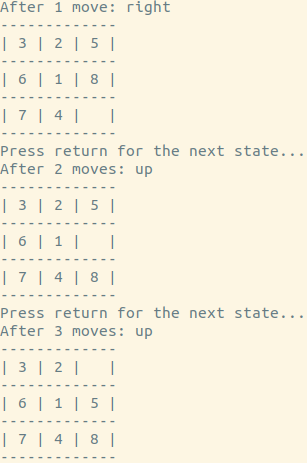
\includegraphics[height=0.45\textwidth]{./img/ex2/8p_1}} 
    \subfigure[]{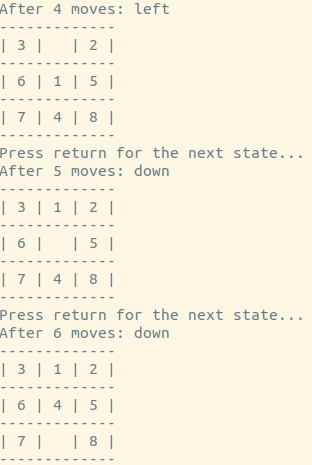
\includegraphics[height=0.45\textwidth]{./img/ex2/8p_2}} 
    \subfigure[]{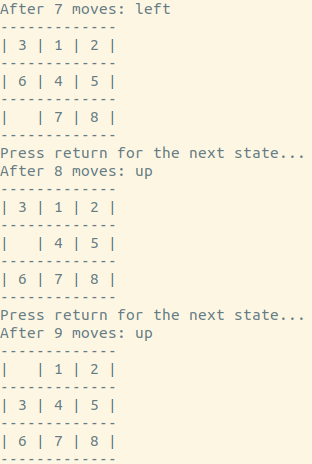
\includegraphics[height=0.45\textwidth]{./img/ex2/8p_3}}
    \caption{Execution of the eightpuzzle}
    \centering
    \label{8p}
\end{figure}

\begin{figure}[H]
    \centering
    \subfigure[]{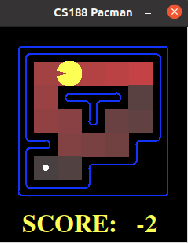
\includegraphics[height=0.29\textwidth]{./img/ex2/BFStiny}} 
    \subfigure[]{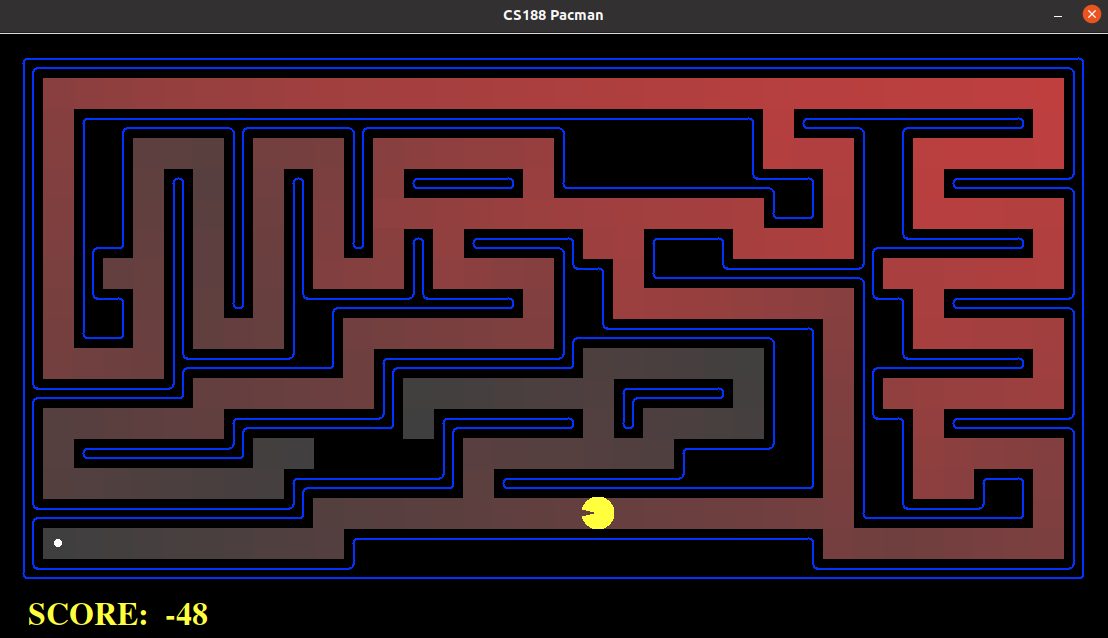
\includegraphics[height=0.29\textwidth]{./img/ex2/BFSmedium}} 
    \subfigure[]{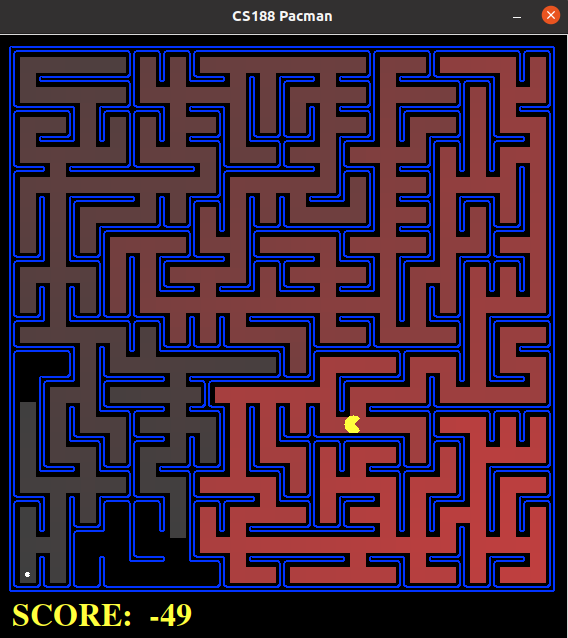
\includegraphics[height=0.29\textwidth]{./img/ex2/BFSbig}}
    \caption{Exploration for mazes with \emph{BFS}: \emph{tinyMaze}, \emph{mediumMaze} and \emph{bigMaze}.}
    \centering
    \label{exploration_e2}
\end{figure}

\myFigure{./img/ex2/test2}{Results of the autograder tests}{test2}{.7}

\subsection{Conclusions on the behavior of Pacman, it is optimal (y/n), reaches the solution (y/n), nodes that it expands, etc (0.5pt)}
\subsubsection{Answer to question 3: Does BFS find a least cost solution? If not, check your implementation.}

BFS algorithm does not expand to height $h+1$ until all nodes of height $h$ have been explored. Thus, the solution obtained has to be the one with minimum height; in other words, the shortest path.

\pagebreak
\section{Question 3: }

\subsection{Personal comment on the approach and decisions of the proposed solution (0.5pt)}

We have implement the \textit{UCS} search as an \textit{A*} search where the heuristic is the trivial one ($h\equiv0$). Therefore we only take into account the total cost to reach a node from the root.

\subsubsection{List \& explanation of the framework functions used}

\begin{itemize}
    \item \texttt{uniformCostSearch(problem)}
\end{itemize}

As mentioned before, we have used the function for \textit{A*} search which, once again, uses the generic function \texttt{search()}. In the next section, we will cover with more detail the function \texttt{aStarSearch()}. The `null heuristic' is a function already given.

\subsubsection{Includes code written by students}


\begin{lstlisting}[language=python,captionpos=t,caption={The \emph{UCS} function (\emph{search.py})}]
    def uniformCostSearch(problem):
        """Search the node of least total cost first."""
        return aStarSearch(problem, nullHeuristic)
\end{lstlisting}


\subsubsection{Screenshots of executions and test carried out analyzing the results}

\myFigure{./img/ex3/victoryUCS}{Results of the three tests using UCS}{victoryBFS}{.8}

\pagebreak

\begin{figure}[h!]
    \centering
    \subfigure[]{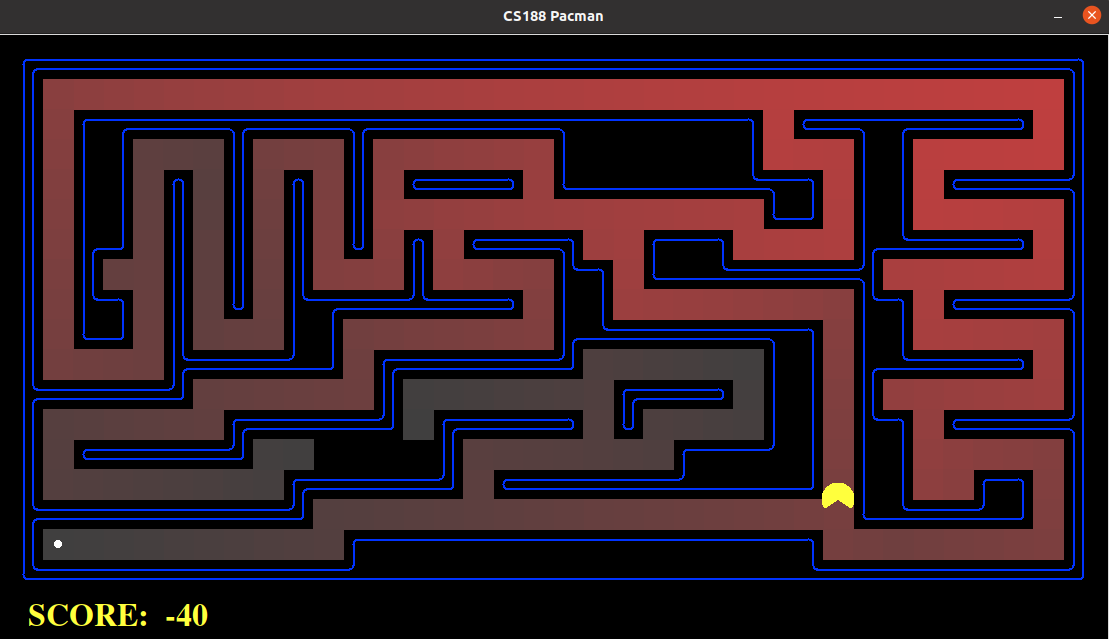
\includegraphics[width=0.65\textwidth]{./img/ex3/medium}} 
    \subfigure[]{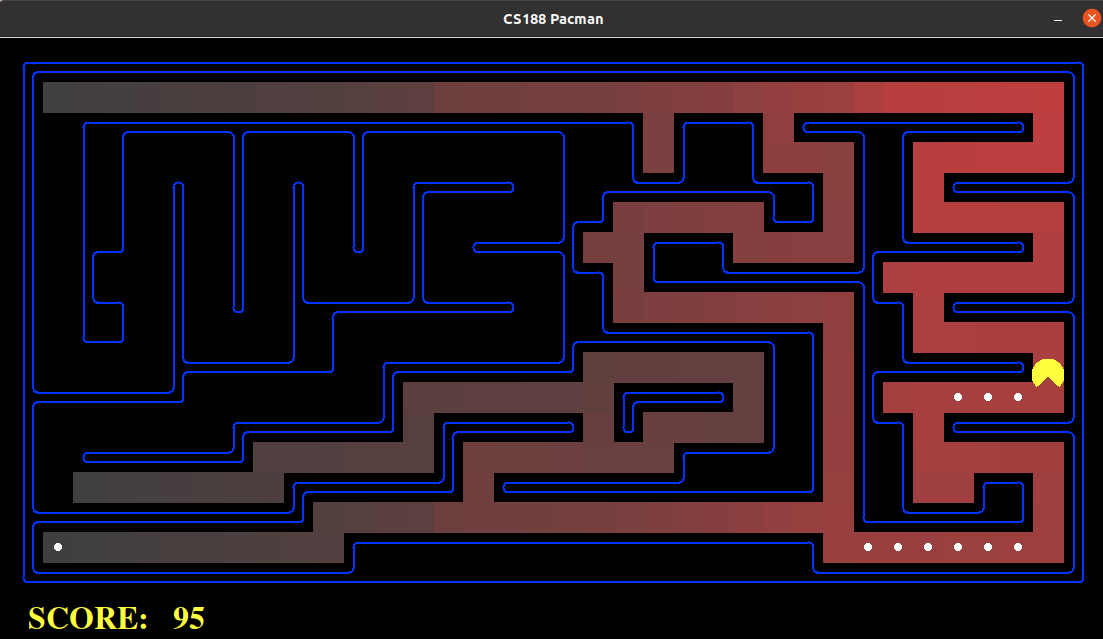
\includegraphics[width=0.65\textwidth]{./img/ex3/east}} 
    \subfigure[]{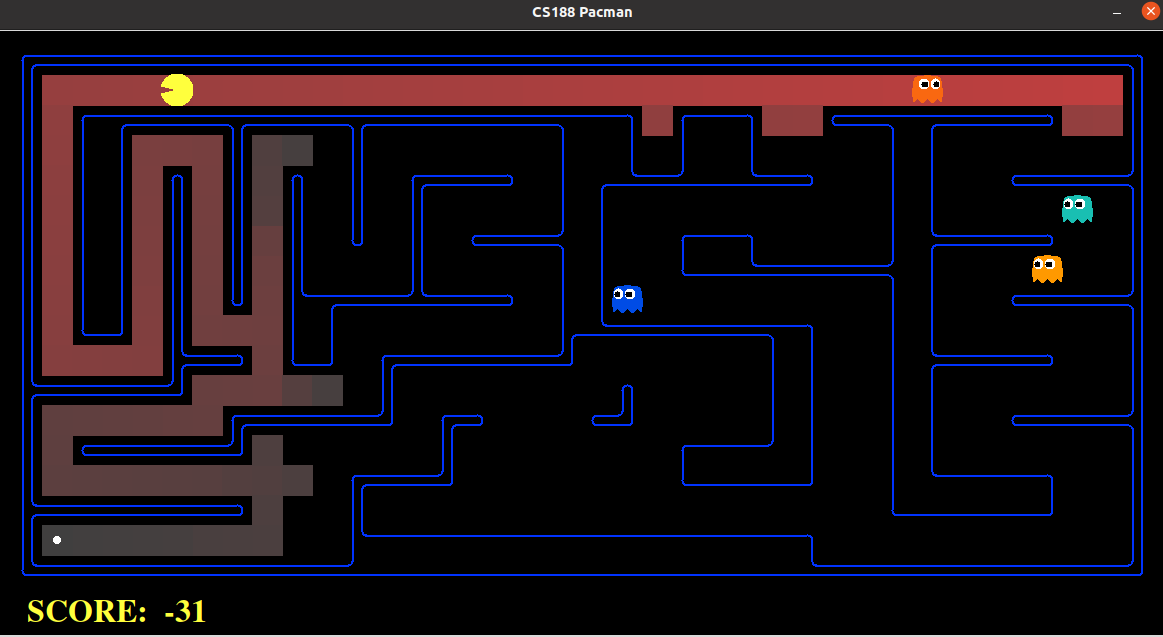
\includegraphics[width=0.65\textwidth]{./img/ex3/west}}
    \caption{Exploration for mazes: (a) \emph{mediumMaze} with \emph{UCS}, (b) \emph{mediumDottedMaze} with \emph{StayEastSearchAgent}, (c) \emph{mediumScaryMaze} with \emph{StayWestSearchAgent}}
    \centering
    \label{exploration_e3}
\end{figure}

\pagebreak

\myFigure{./img/ex3/test3}{Results of the autograder tests}{test3}{.75}

\pagebreak

\subsection{Conclusions on the behavior of Pacman, it is optimal (y/n), reaches the solution (y/n), nodes that it expands, etc (0.5pt)}

Uniform cost search is always optimal in terms of the cost defined. Thus, executing \textit{UCS} assigning a cost of 1 to all the edges, results on a solution of minimum length. However, if the agents \texttt{StayWestSearchAgent()} or \texttt{StayEastSearchAgent()} are used, the solution is not the shortest because this time, the cost function does not represent length of the path to a node but longitude of its position.


\pagebreak
\section{Question 4: }

\subsection{Personal comment on the approach and decisions of the proposed solution (1pt)}

The algorithm for \textit{A*} is just the same as for the other search types. The only difference, as expected, is the way we extract nodes from the \emph{openList}. Thus, we have reused our generic search function once again.

\subsubsection{List \& explanation of the framework functions used}

\begin{itemize}
    \item \texttt{aStarSearch(problem)}
\end{itemize}

The container used for this search is a priority queue (\textit{PriorityQueueWithFunction}) where the priority is defined by the evaluation function which is the sum between the cost to reach the node and the heuristic value of it. This function is defined on the fly using a lambda expression.

\subsubsection{Includes code written by students}

\begin{lstlisting}[language=python,captionpos=t,caption={The \emph{A*} function (\emph{search.py})}]
    def aStarSearch(problem, heuristic=nullHeuristic):
        """Search the node that has the lowest combined cost and heuristic first."""
        return search(problem, 
                      util.PriorityQueueWithFunction(
                        lambda node: node.cost + heuristic(node.state, problem)))
\end{lstlisting}


\subsubsection{Screenshots of executions and test carried out analyzing the results}

\myFigure{./img/ex4/victoryAS}{Results of the test using \emph{A*}}{victoryAS}{1}

\myFigure{./img/ex4/ASbig}{Exploration of the maze from previous execution}{victoryAS}{.4}

\myFigure{./img/ex4/test4}{Results of the autograder tests}{test4}{.7}

\subsection{Conclusions on the behavior of Pacman, it is optimal (y/n), reaches the solution (y/n), nodes that it expands, etc (1pt)}

As we know from theory, \textit{A*} with elimination of repeated states is optimal if the heuristic used is admissible and consistent. For the position problem, the \emph{ManhattanHeuristic} satisfies both conditions. If we consider a relaxation of the problem, a maze with no walls, the optimal path has exactly the length given by the Manhattan metric. It is also consistent because the cost of going from a node to one of its successor is always equal to 1, and at most, the successor will be one tile closer to the solution, (it may be 1 tile farther too). In other words, the following inequality holds:

\begin{equation}
    \begin{split}
    \forall n,n':n' \text{ succesor of }n \text{, }
    h(n) \leq \text{cost}(n \rightarrow n')+h(n') 
    \label{consistent}
    \end{split}
\end{equation}

Indeed, as this heuristic is consistent, it immediately follows that it is also admissible.


\subsubsection{Answer to question 4: What happens on openMaze for the various search strategies?}

\myFigure{./img/ex4/openMaze}{Execution for the four strategies in the \emph{openMaze}.}{openMaze}{.9}

The layout \emph{openMaze} has almost no walls so the perfomance of \textit{DFS} (which is not an optimal algorithm) will be determined by the order of how the successors are generated. Just for instance, with the order \texttt{(NORTH,SOUTH,EAST,WEST)}, the solution has a length of 298 and 576 are expanded. However if we change the order to \texttt{(EAST,SOUTH,NORTH,WEST)}, the solution has a cost of 54 and the expanded nodes are 247. 

\myFigure{./img/ex4/openMaze_dif_order}{\emph{BFS} with the order of successor selection: \texttt{(EAST,SOUTH,NORTH,WEST)} in \emph{openMaze}.}{openMaze2}{.8}

On the other hand, we know that \textit{BFS}, \textit{UCS} and \textit{A*} (with a consisten heuristic), will provide an optimal solution. Nonetheless, the number of nodes expanded vary.  
\textit{BFS} and \textit{UCS} do not take into account how close a position is from the solution, therefore nodes are expanded only taking into account the cost of reaching them. However, if we introduce the Manhattan heuristic into the calculation, we can ensure that nodes which are further from the solution will only be explored when it is the only available way. So, to sum up, using a consistent heuristic will result in reaching an optimal solution and generally with a lower number of nodes expanded. It is worth mentioning that less nodes expanded may not always result in less computing time.


\pagebreak
\section{Question 5: Finding All the Corners}

\subsection{Personal comment on the approach and decisions of the proposed solution (1pt)}

For this problem (\emph{CornersProblem}) we have chosen the following state representation: 
\begin{equation}
s = (s_p, s_c)\text{,}
\label{state}
\end{equation}
where $s_p$ is the 2-tuple that denotes the position of Pacman (coordinates as defined in the \emph{Grid} class --which must be a legal position) in the corners problem; and $s_c$ is the set of corners (their coordinates) that have yet not been visited by Pacman. We have chosen to keep track of the unvisited corners instead of the visited ones because it makes easier the computations of the heuristic for the next section.

For the problem class itself, it is quite similar to the \emph{PositionProblem} class but we have added two new atributes (\emph{shortSide} and \emph{longSide}) which hold the size of the maze (the distances between adjacent corners). These attributes are used in our heuristic of the next section.

\subsubsection{List \& explanation of the framework functions used}

\begin{itemize}
    \item The \texttt{CornersProblemState} class, with methods:
    \begin{itemize}
        \item \texttt{\_\_init\_\_(self, position, remainingTargets)}
        \item \texttt{\_\_eq\_\_(self, \_\_o)}
    \end{itemize}
    \item The \texttt{CornersProblem} class, with methods:
    \begin{itemize}
        \item \texttt{\_\_init\_\_self, startingGameState)}
        \item \texttt{getStartState(self)}
        \item \texttt{isGoalState(self, state)}
        \item \texttt{getStartState(self)}
        \item \texttt{getSuccessors(self, state)}
    \end{itemize}
    \item \texttt{expandNode(problem , node , openList , closedList)}
    \item \texttt{search(problem, openList)}
    \item \texttt{depthFirstSearch(problem)}
\end{itemize}

For this section we had to complete the \emph{CornersProblem} class, so that this problem had appropriate states and the successors were calculated according to the defined problem.

\subsubsection{Includes code written by students}

\begin{lstlisting}[language=python,captionpos=t,caption={The state and problem definition of the corners problem (\emph{searchAgents.py})}]
    CORNERS_PROB_ACTION_COST = 1

    class CornersProblemState():
        '''
            The state of the corners problem.
                position: (x,y) - position in the game
                remainingTargets: (list of) remaining targets (positions) 
                to solve the game - (it is not possible to have the position 
                of a state inside its own remainingTargets, this initialization
                takes care of that)
        '''
        def __init__(self, position, remainingTargets):
            self.position = position
            self.remainingTargets = remainingTargets.copy()
            if position in remainingTargets:
                self.remainingTargets.remove(position)
        
        def __eq__(self, __o):
            if isinstance(__o, CornersProblemState):
                return (__o.position == self.position) \
                        and (set(__o.remainingTargets) == set(self.remainingTargets)) 
            return False

    class CornersProblem(search.SearchProblem):
        """
        This search problem finds paths through all four corners of a layout.

        You must select a suitable state space and successor function
        """

        def __init__(self, startingGameState):
            """
            Stores the walls, Pacman's starting position and corners.
            """
            self.walls = startingGameState.getWalls()
            self.startingPosition = startingGameState.getPacmanPosition()
            top, right = self.walls.height-2, self.walls.width-2
            self.corners = ((1,1), (1,top), (right, 1), (right, top))
            for corner in self.corners:
                if not startingGameState.hasFood(*corner):
                    print('Warning: no food in corner ' + str(corner))
            self._expanded = 0 # DO NOT CHANGE; Number of search nodes expanded
            # Please add any code here which you would like to use
            # in initializing the problem

            self.startState = CornersProblemState(self.startingPosition, list(self.corners))
            self.shortSide = min(self.walls.height,self.walls.width)-3
            self.longSide = max(self.walls.height,self.walls.width)-3

        def getStartState(self):
            """
            Returns the start state (in your state space, not the full Pacman state
            space)
            """
            return self.startState

        def isGoalState(self, state):
            """
            Returns whether this search state is a goal state of the problem.
            """
            return not state.remainingTargets

        def getSuccessors(self, state):
            """
            Returns successor states, the actions they require, and a cost of 1.

            As noted in search.py:
                For a given state, this should return a list of triples, (successor,
                action, stepCost), where 'successor' is a successor to the current
                state, 'action' is the action required to get there, and 'stepCost'
                is the incremental cost of expanding to that successor
            """

            successors = []
            for action in [Directions.NORTH, Directions.SOUTH, Directions.EAST, Directions.WEST]:
                "*** YOUR CODE HERE ***"
                x,y = state.position
                dx, dy = Actions.directionToVector(action)
                nextx, nexty = int(x + dx), int(y + dy)
                if not self.walls[nextx][nexty]:
                    nextState = CornersProblemState((nextx,nexty),state.remainingTargets)                
                    cost = CORNERS_PROB_ACTION_COST
                    successors.append((nextState, action, cost))

            self._expanded += 1 # DO NOT CHANGE
            return successors
\end{lstlisting}

Note: the \texttt{getCostOfActions} method from the \emph{CornersProblem} class has not been included, because we did not have to modify it. 

\subsubsection{Screenshots of executions and test carried out analyzing the results}

\myFigure{./img/ex5/victoryCorners}{Results of the two corner tests}{victoryCorners}{1}

\begin{figure}[h!]
    \centering
    \subfigure[]{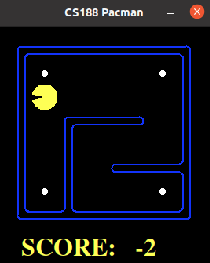
\includegraphics[height=0.3\textwidth]{./img/ex5/tiny}} 
    \subfigure[]{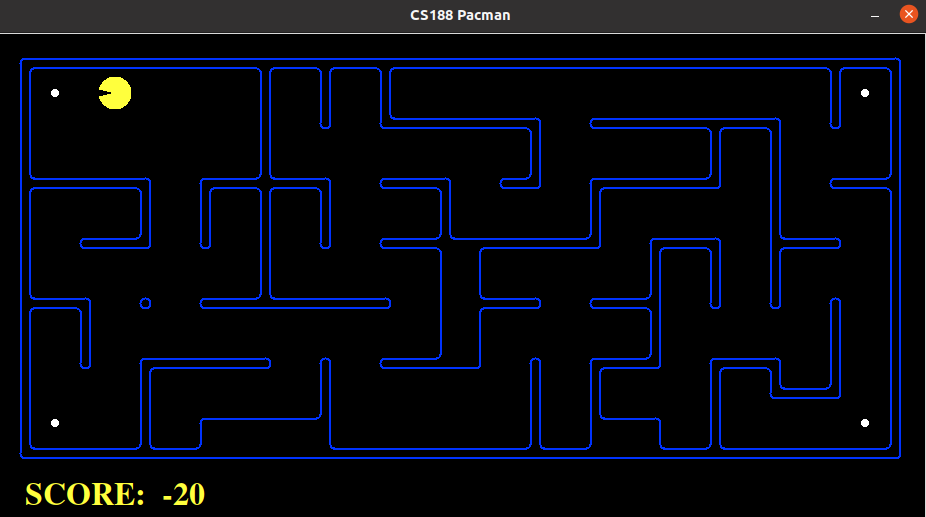
\includegraphics[height=0.3\textwidth]{./img/ex5/medium}}
    \caption{Execution of the (a) \emph{tinyCorners} maze and the (b) \emph{mediumCorners} maze.)}
    \centering
    \label{corners_execution}
\end{figure}

\myFigure{./img/ex5/test5}{Results of the autograder tests}{test5}{.7}


\subsection{Conclusions on the behavior of Pacman, it is optimal (y/n), reaches the solution (y/n), nodes that it expands, etc (1pt)}

Pacman reaches the solution in all tests. The fact that this is a different problem does not change the way the algorithms find solutions; therefore, the comments made in previous sections about each algorithm still hold in this problem. \emph{BFS} is optimal.



\pagebreak
\section{Question 6: Corners Problem: Heuristic}

\subsection{Personal comment on the approach and decisions of the proposed solution (1.5pt)}

\subsubsection{List \& explanation of the framework functions used}

\begin{itemize}
    \item \texttt{minCornerTravel(numCorners, remainingCorners, shortSide, longSide)}
    \item \texttt{cornersHeuristic(state, problem)}
\end{itemize}

In this section, we only had to complete the \texttt{cornersHeuristic} function. 

We also used the \texttt{util.manhattanDistance()} function to calculate some distances. 

\subsubsection{Includes code written by students}

\begin{lstlisting}[language=python,captionpos=t,caption={The heuristic definition (\emph{searchAgents.py})}]
    def minCornerTravel(numCorners, remainingCorners, shortSide,longSide):
        '''
        Returns the distance that Pacman would travel (starting from one of the 
        remaining corners and ending in the last remaining corner) in the corners 
        problem if there were no internal walls, and starting form the corner that 
        makes this distance the minimum.
            numCorners: the length of remaining corners
            remainingCorners: the remaining corners to visit
            shortSide: the length of the short side of the grid 
            longSide: the length of the long side of the grid
        '''
        if numCorners == 1:
            return 0
        if numCorners == 2:
            return util.manhattanDistance(remainingCorners[0],remainingCorners[1])
        if numCorners == 3:
            return shortSide + longSide
        return 2*shortSide + longSide

    def cornersHeuristic(state, problem):
        """
        A heuristic for the CornersProblem that you defined.

        state:   The current search state
                (a data structure you chose in your search problem)

        problem: The CornersProblem instance for this layout.

        This function should always return a number that is a lower bound on the
        shortest path from the state to a goal of the problem; i.e.  it should be
        admissible (as well as consistent).
        """
        if not state.remainingTargets:
            return 0

        nearestCornerDistance = min(
            [util.manhattanDistance(state.position, c) 
                for c in state.remainingTargets]
        )    
        minDistanceBetweenCorners = minCornerTravel(
            len(state.remainingTargets), 
            state.remainingTargets, 
            problem.shortSide,
            problem.longSide
        )
        return nearestCornerDistance + minDistanceBetweenCorners
\end{lstlisting}

\subsubsection{Screenshots of executions and test carried out analyzing the results}

\myFigure{./img/ex6/victoryCornersAS}{Results of the test using \emph{A*} for the corners problem.}{victoryCornersAS}{1}

\myFigure{./img/ex6/ASmedium}{Exploration of the maze from previous execution}{victoryAS}{.5}

\myFigure{./img/ex6/test6}{Results of the autograder tests}{test6}{.9}

\subsection{Conclusions on the behavior of Pacman, it is optimal (y/n), reaches the solution (y/n), nodes that it expands, etc (1.5pt)}

This implementation is optimal, because it uses \emph{A*}, with elimintation of repeated states, and a consistent heuristic (proof in the next subsection). It also reaches the solution, and expands 774 nodes in the \emph{mediumCorners} maze.

\subsubsection{Answer to question 5: Explain the logic behind your heuristic}

For the heuristic, we have solved the cost of the problem with a relaxation: there are no internal walls. In the case of 3 remaining corners, there is also another relaxation: we assume that Pacman is closest to one of the 2 corners that are opposite in the grid. This second relaxation could be solved by complicating the heuristic a little, but we have observed that it is not worth the computational cost it adds, taking into account that the improvement in terms of explorated nodes is not significant. 


Notation: we will use $d$ to denote the Manhattan Distance (in this case, in $(\mathbb{N}\cup \{0\})^2\times (\mathbb{N}\cup \{0\})^2$). 

\begin{equation}
    d((x_1,x_2),(y_1,y_2)) = |y_1-x_1| + |y_2-x_2|
\end{equation}

The heuristic chosen ($h$) has been defined as follows: given a state $s$, as defined in \ref{state}, we define:

\begin{equation}
    h_1(s) = \left\{ \begin{array}{lcc}
        0 &   \text{if}  & |s_c| = 0 \\
        \min \{d(s_p, c):c\in s_c\} &   \text{if}  & |s_c| > 0 \\
        \end{array}
        \right\}
\end{equation}

This $h_1$ function calculates the minimum distance from Pacman's position to a corner that has not been visited.

\begin{equation}
    h_2(s) = \left\{ \begin{array}{lcc}
        0 &   \text{if}  & |s_c| \leq 1 \\
        d(c_1,c_2)\text{, where } \{c_1,c_2\}=s_c &   \text{if}  & |s_c| = 2 \\
        m+M &   \text{if}  & |s_c| = 3 \\
        2m+M &   \text{if}  & |s_c| = 4 \\
        \end{array}
        \right\}\text{,}
\end{equation}

where $m = \min S$ and $M = \max S$, $S=\{\text{distances between any two adjacent corners in the grid}\}$. 

Finally, 

\begin{equation}
    h(s) = h_1(s)+h_2(s)
\end{equation}

We will now prove that $h$ is consistent, i.e. that for each node $s$ and for each successor $s'$ of $s$, $h(s) \leq \text{cost}(s,s') + h(s') = 1 + h(s')$. (The cost is always 1, from any node to any of its successors).
\bigskip
\begin{tcolorbox}[breakable, enhanced]
\begin{proof}

    The proof will be separated into two cases.

    \begin{enumerate}
        \item Case $s_c = s'_c$, this happens if $s'_p$ is not a corner. By definition of $h_2$, in this case, $h_2(s)=h_2(s')$. To be proven: $h_1(s) \leq h_1(s')+1$:
        \begin{enumerate}
            \item If $|s_c| = 0$, the $s$ is a goal state and has no succesors.
            \item If $|s_c|>0$; $h_1(s)=d(s_p,c_0)$ and $h_1(s')=d(s'_p,c_1)$, for $c_0,c_1\in s_c=s'_c$.
            Also, $d(s_p,s'_p)=1$. So (triangle inequality): 
                $$d(s_p,c_1)\leq 1+d(s'_p,c_1)$$
                $$d(s'_p,c_1)\leq 1+d(s_p,c_1)$$
                $$\Rightarrow -1\leq d(s_p,c_1)-d(s'_p,c_1)\leq 1$$
                $$\Rightarrow \exists k\in \{-1,0,1\}:d(s_p,c_1)=d(s'_p,c_1)+k$$
                $$\Rightarrow h_1(s)= d(s_p,c_0)\leq d(s_p,c_1) = d(s'_p,c_1)+k\leq d(s_p',c_1)+1 = h_1(s')+1$$
        \end{enumerate}
        \item Case $s_c \neq s'_c$, this happens if $s'_p$ is a corner. In this case, $h_1(s) = 1$.
        \begin{enumerate}
            \item If $|s_c|=0$ (again, this does not make much sense, because the algorithm would stop before evaluating successors of $s$ if $s$ is a goal state, and we have defined goal states as those whose remaining targets-set is empty).
            \item If $|s_c|=1$, then $|s'_c|=0$, so $h(s')=0$, and $h(s)=1\leq 1+h(s')=1$
            \item If $|s_c|=2$, then $|s'_c|=1$. $s_c=\{s'_p,c_1\}$, $s'_c=\{c_1\}$. $h(s)=1+d(s'_p,c_1)=1+h(s')$
            \item If $|s_c|=3$, then $|s'_c|=2$. $s_c=\{s'_p,c_0,c_1\}$, $s'_c = \{c_0, c_1\}$. 
            
            So $h(s)=1+m+M$. And $h(s') =\min \{d(s'_p,c_0),c(s'_p,c_1)\} + d(c_0,c_1)$. It is easy to see that if $\{s'_p,c_0,c_1\}$ are three different corners, $\min \{d(s'_p,c_0),c(s'_p,c_1)\} + d(c_0,c_1) \geq m+M$. Therefore, $h(s)\leq 1+m+M\leq 1+h(s')$.
            \item If $|s_c|=4$, then $|s'_c|=3$. For a corner $c_0\in s'_c$, $h_1(s')=d(s'_p,c_0)\geq m$. 
            
            Then $h(s')=d(s'_p,c_0)+m+M\geq 2m + M = h(s) - 1$
        \end{enumerate}
    \end{enumerate}
\end{proof}
\end{tcolorbox}


\section{Question 7: Personal comments on the development of this practice.}

During these exercises, we have tried to develop code that not only solved the Pacman game but any other defined-state (single player) game by generalizing the functions and by abstraction. One example of this can be found in \textit{search.py} where the different search methods are performed with the same algorithm, changing only the data structure where the discovered nodes are added and later on, popped to be expanded. Moreover, the class \textit{Node} is an example of our intention to make an abstraction of the problem. While the code provided used a 3-tuple to encode succesors, we have avoided these kind of tuples for legitibility sake.

On the other hand, the only part of the assigment where we actually have had to consider the features of the Pacman was when coding the heuristic for the corners problem. Indeed, the only assumption needed was the maze being a rectangle (or square). Talking about the heuristic, our approach was to consider the four different scenarios of how many corners could remain unvisited. The advantage of breaking the heuristic into cases (divide \& conquer) is that any modification to make a more complex heuristic (like considering if Pacman's way out is blocked when only one corner is left) would have been easier to implement. From the four scenarios, the case of having three remaining corners was the one that presented more possibilities of implementation. As mentioned in the previous section, our approach (that considers the most favorable case) gave very similar results to other implementations we tried while making less computations. So at the end, it resembled to many other situations where the decisions are down to a cost vs perfomance trade-off.

\end{document}

